% Document parameters
\title{Template Assignment} % EDIT THIS
\author{Your Name, StudentNo.} % EDIT THIS

% General imports
\documentclass[12pt]{article}
\usepackage[english]{babel}
\usepackage[utf8]{inputenc}

\usepackage{url}
\usepackage{hyperref}

\usepackage{booktabs}
\usepackage{amsmath}
\usepackage{amssymb}

\usepackage{calc}
\usepackage{enumitem}

\usepackage{graphicx}
\graphicspath{{images/}} % Images are being fetched from the images sub directory.

% Bibliography imports
\usepackage{biblatex}
\addbibresource{bibtex.bib}

% Title (and page header)
\usepackage{fancyhdr}
\usepackage{titlesec}
\usepackage{vmargin}
\setmarginsrb{3 cm}{2.5 cm}{3 cm}{2.5 cm}{1 cm}{1.5 cm}{1 cm}{1.5 cm}

\makeatletter
\let\thedoctitle\@title
\makeatother

\pagestyle{fancy}
\lhead{\thedoctitle}
\rhead{}
\cfoot{\thepage}

\begin{document}

\begin{titlepage}
	\maketitle
    \thispagestyle{empty}
\end{titlepage}

\section{Image placement}\label{sec:image-placement}
Bacon ipsum dolor amet flank pork pork chop, tri-tip ham turkey shank ground round jerky tail landjaeger sausage brisket. Fatback turkey short ribs beef ribs buffalo kevin jowl hamburger leberkas. Flank spare ribs venison, ball tip prosciutto t-bone beef shankle ground round. Andouille boudin shoulder corned beef pork chop swine.

\begin{figure}[h] % [h] places the image between the text
    \centering
    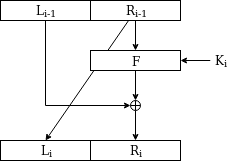
\includegraphics[scale=0.75]{example.png} % Scale the image to size
    \caption{Example caption}
    \label{fig:example}
\end{figure}

Bacon rump turducken jowl burgdoggen picanha brisket boudin pork belly capicola kevin pig strip steak landjaeger. Porchetta fatback short ribs meatball tongue. Beef boudin bacon, venison pork chop chuck shank shoulder swine buffalo salami pork porchetta shankle meatball. Frankfurter pig swine tail cow, prosciutto pork loin alcatra. Picanha cupim jowl, brisket burgdoggen jerky tri-tip rump ham kielbasa bresaola frankfurter drumstick.

\section{Tables}
\begin{table}[h] % Add [h] after generation
\centering % Add after generation
\begin{tabular}{@{}ll@{}}
\toprule
\textbf{$x$} & \textbf{$p(P=x)$} \\ \midrule
a            & 2/7               \\
b            & 1/7               \\
c            & 3/7               \\
d            & 1/7               \\ \bottomrule
\end{tabular}
\caption{Example caption} % Add after generation
\label{tab:example} % Add after generation
\end{table}

Table \ref{tab:example} generated using \url{https://www.tablesgenerator.com/latex_tables} \newline (booktabs table style).

\section{Text formatting}
\begin{itemize}
    \item \textbf{Bold} \textit{}
    \item \textit{Italic}
    \item \texttt{Typewriter}
    \item Formula: $f(\alpha) = \frac{\beta}{\gamma}$
\end{itemize}

\section{Enumeration}
\subsection{Normal enumeration}
\begin{enumerate}
    \item One
    \item Two
    \item Three
\end{enumerate}

\subsection{Special enumeration}
\begin{enumerate}[label=(\alph*.)]
    \item One
    \item Two
    \item Three
\end{enumerate}

\subsection{Descriptions}
\begin{description}
    \item[Not very meaty] text
    \item[Meaty] Shankle pig fatback chicken, hamburger sausage shoulder pork chop brisket flank cow rump tri-tip. Pork loin rump jerky pork chop ham hock shank.
\end{description}

\subsection{Aligned descriptions}
\begin{description}[leftmargin=!,labelwidth=\widthof{\bfseries Not very meaty}] 
% Change \widthof to the longest label. Warnings will occur if this is set incorrectly.
  \item[Not very meaty] text
  \item[Meaty] Salami pastrami prosciutto beef alcatra burgdoggen pork. Meatloaf landjaeger tail, leberkas rump tenderloin salami drumstick burgdoggen picanha tri-tip short loin brisket.
\end{description}

\section{References}
In Section \ref{sec:image-placement}, we observe Figure \ref{fig:example}. Clicking these reference numbers will show the referred part of the document.

\section{Citations}
Lets cite \cite{einstein}, APA style. You can add citations in bibtex.bib. Citations will show up in the references section only if you cited them using the cite command.

\printbibliography

\end{document}